\documentclass{thureport}
% =============================================
% Part 1 Edit the info
% =============================================

\newcommand{\major}{软件71}
\newcommand{\name}{骆炳君}
\newcommand{\stuid}{2017013573}
\newcommand{\newdate}{2019-4-25}
\newcommand{\newtitle}{逸出功的测量}
\newcommand{\dL}{\delta L}
\def\celsius{{\ensuremath{^\circ\hspace{-0.09em}\mathrm{C}}}}

% =============================================
% Part 1 Main document
% =============================================
\begin{document}
\thispagestyle{empty}
\begin{figure}[h]
	\begin{minipage}{0.65\linewidth}
		\centerline{
\includegraphics[width=\linewidth]{head.jpg}}
	\end{minipage}
	\hfill
	\begin{minipage}{.3\linewidth}
		\raggedleft
		\begin{tabular*}{.8\linewidth}{ll}
			班级: & \underline\major   \\
			姓名: & \underline\name    \\
			学号: & \underline\stuid   \\
			日期: & \underline\newdate
		\end{tabular*}
	\end{minipage}
\end{figure}

\begin{table}[!htbp]
	\centering\large
	实验名称: \underline\newtitle
\end{table}

\tableofcontents
% =============================================
% Part 2 Main document
% =============================================
\newpage

\section{实验目的}
\begin{clause}
	\item 学习用里查孙直线法测定阴极材料的电子逸出功.
	\item 了解热电子发射规律和现象.
	\item 学习针对难以测量的物理量的处理方法.
\end{clause}

\section{数据处理}
\subsection{电路图}
\begin{figure}[h]
	\centering
	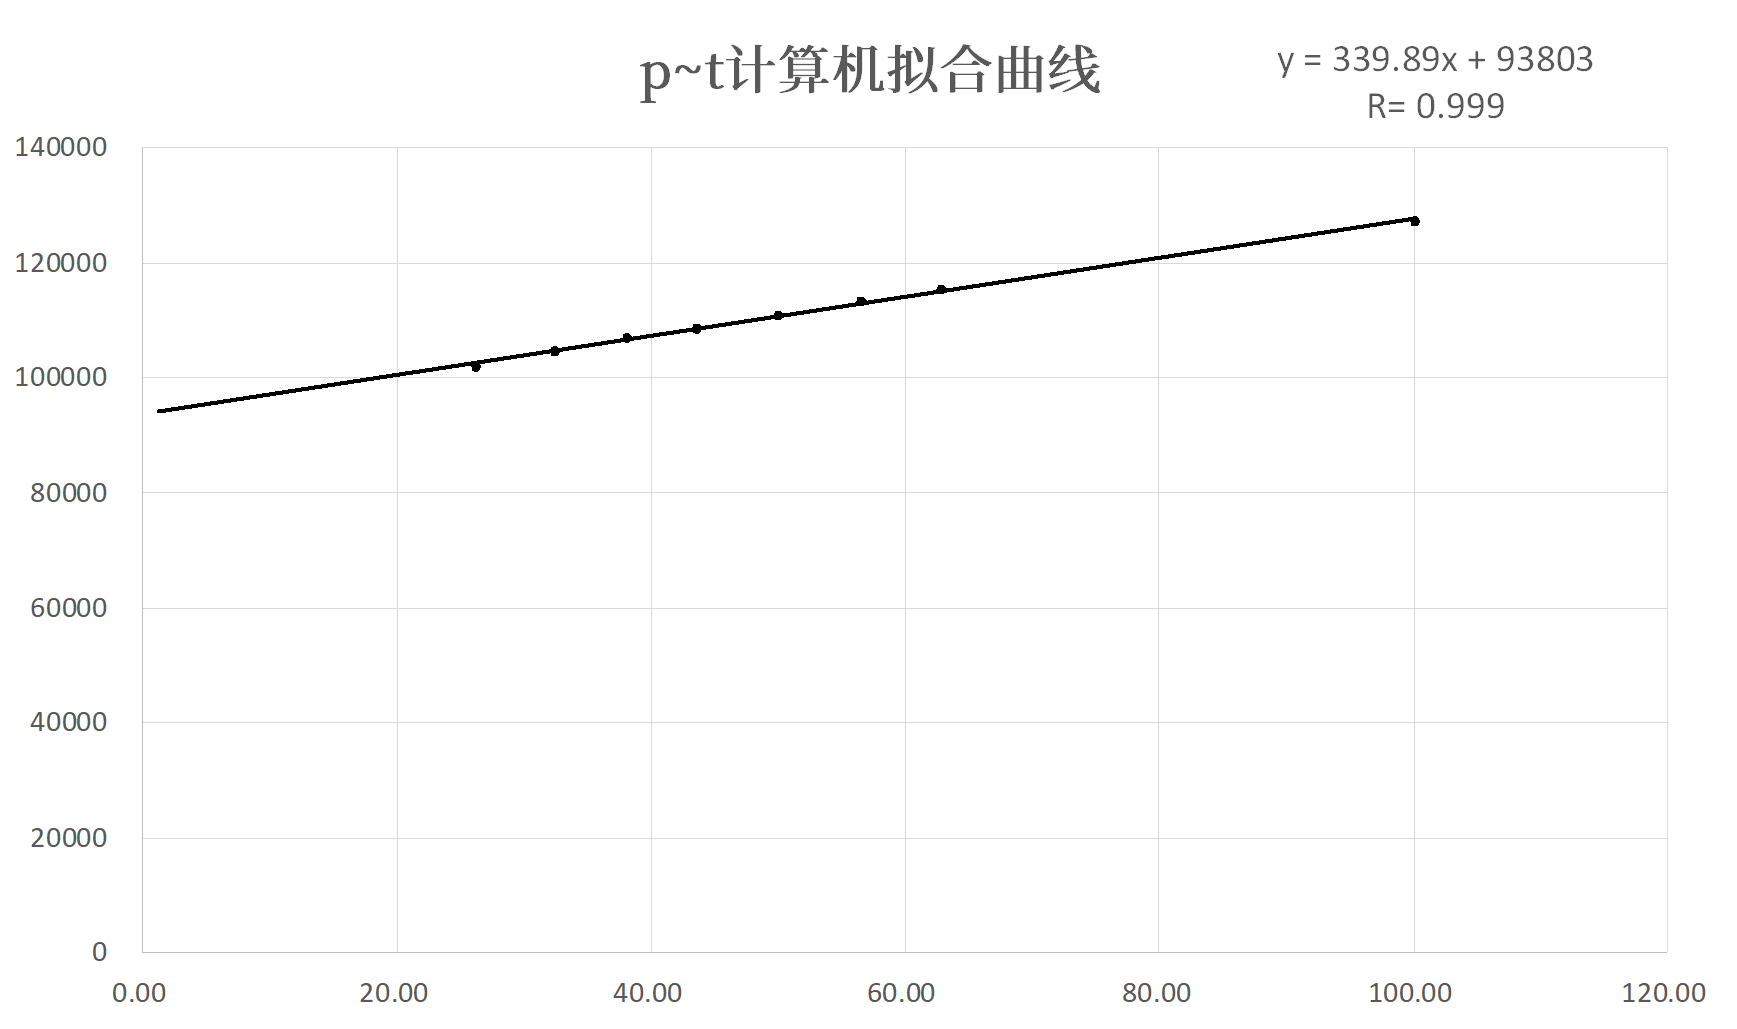
\includegraphics[width=0.9\linewidth]{figure3.png}
\end{figure}

\subsection{不同温度$T$下的$\lg{U_e'}\sim \sqrt{U_a}$直线拟合}
通过调节通过钨丝的电流来调节温度$T$,测量不同$T$下的$U_e'$和$U_a$,经过直线拟合(见附图)得到以下数据:

\begin{table}[H]
    \centering
      \begin{tabular}{|c|c|c|c|}
      \hline
      $I_f$/A & $T$/K & 截距$\lg{U_e}$ & $U_e/V$ \bigstrut\\
      \hline
      0.502 & 1729.32 & 0.904517 & 2.470739 \bigstrut\\
      \hline
      0.544 & 1799.04 & 1.468202 & 4.341424 \bigstrut\\
      \hline
      0.581 & 1869.04 & 1.980184 & 7.244075 \bigstrut\\
      \hline
      0.624 & 1936.52 & 2.420013 & 11.246 \bigstrut\\
      \hline
      0.662 & 1995.16 & 2.825889 & 16.87593 \bigstrut\\
      \hline
      0.702 & 2062.08 & 3.183054 & 24.12031 \bigstrut\\
      \hline
      \end{tabular}%
  \end{table}%

\subsection{$\lg{\frac{U_e}{T^2}}\sim\frac{1}{T}$直线拟合}
由实验讲义表格使用直线插值法可求出钨丝温度$T$,得到以下数据:
% Table generated by Excel2LaTeX from sheet 'Sheet4'
\begin{table}[H]
    \centering
      \begin{tabular}{|c|c|c|c|c|c|c|}
      \hline
      $T$/K & 1729.32 & 1799.04 & 1869.04 & 1936.52 & 1995.16 & 2062.08 \bigstrut\\
      \hline
      $\frac{1}{T}/K^{-1}$ & 0.000578 & 0.000556 & 0.000535 & 0.000516 & 0.000501 & 0.000485 \bigstrut\\
      \hline
      $\lg{\frac{U_e}{T^2}}$ & -5.57123 & -5.04188 & -4.56305 & -4.15403 & -3.77407 & -3.44556 \bigstrut\\
      \hline
      \end{tabular}%
  \end{table}%  

使用计算机对数据进行拟合处理(见附图),可得拟合直线方程为
$$\lg{\frac{U_e}{T^2}}=-22876\frac{1}{T}+7.6676,\quad R^2=0.9996$$

相关系数$R$非常接近1,数据拟合程度较好.

\subsection{逸出功的计算}
由直线方程
$$\lg\frac{U_e}{T^2}=\lg{AS}+\lg{R}-5.039\times10^3\frac{\phi}{T}$$

可得
$$\phi=\frac{k}{-5.039\times10^3}=\frac{-22876}{-5.039\times10^3}=4.540(V)$$

所以逸出功
$$W=e\phi=4.540eV$$

\section{实验小结}
本次实验是电学实验,正确连接电路是实验成功的关键,需要我们对实验原理和仪器都有比较深入的了解.在实验过程中暴露了我的很多不足之处,例如实验电路设计出错,对仪器读数不够熟悉等.感谢助教和老师的悉心指导!

\section{思考题}
\subsection*{1. $I_f$系统误差修正的必要性?}
不需要修正,因为有两个$18k\Omega$的电阻串联,其总阻值远大于灯丝的电阻,分流远小于电流表的仪器误差,可以忽略不计.

\subsection*{2. $U_a$系统误差修正的必要性?}
不需要修正,因为$\frac{R_4}{R_5}=1000$,所以$U_a$的测量系统误差为$\frac{1}{1000}$,可以忽略不计.

\subsection*{3. $U_e'$是否必须化成$I_e'$再进行数据处理?}
不需要,因为$U_e'=I_e'R$,$U_e'$仅为$I_e'$的常数倍,而在后续的数据处理中可以得到$\lg\frac{U_e}{T^2}=\lg{AS}+\lg{R}-5.039\times10^3\frac{\phi}{T}$,无需引入$R$即可由直线斜率求出$\phi$,而且化为$I_e'$会引入有效数字带来的误差,使得计算更加繁琐.

\subsection*{4. C点是否为灯丝中点电位等效点?}
C点是灯丝中点电位等效点,因为灯丝可近似看作是均匀材料,C点到灯丝两端的电阻相等,电压相等,所以是中点电位等效点.

\clearpage
\section{拟合曲线}
\begin{figure}[h]
	\centering
	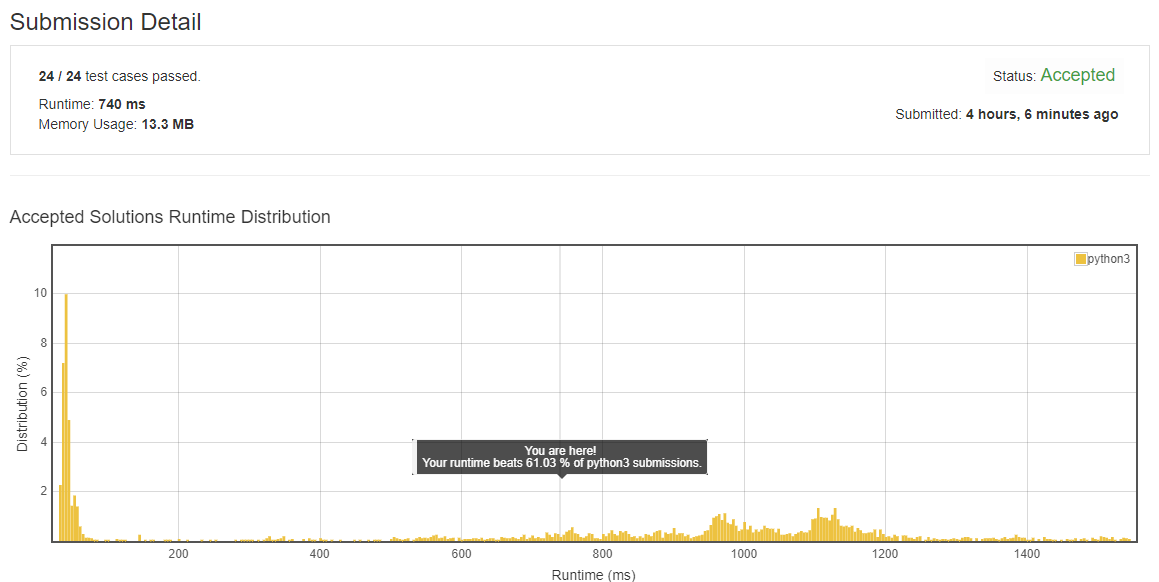
\includegraphics[width=0.9\linewidth]{figure1.png}
\end{figure}
\newpage
\section{原始数据表格}

\end{document}